\chapter{考察}
\label{chap:consideration}

\section{本研究についての考察}
今回作成したシステムを用いることで現状のAndroid Widgetの問題をいくつか解決することができた。
多くのAndroid Widgetを置くことで画面スペースを占有してしまう問題に対しては、情報をテキストとして並べることで省スペースを実現した。
必要な情報に付随して不要な情報も表示されるという問題があったが、ユーザー自身が表示される情報を指定するため、不要な情報は表示されなくなった。
自分の取得したい情報に対応するAndroid Widgetが存在しない場合、自らAndroid Widgetを作成するしか対応策が無かったが、Webページ上のテキストデータやセンシングデータなどを取得可能になった。
これらの面からユーザーに効率良く価値の高い情報を提供するという目的は達成できた。

しかし、今回作成したシステムを実際に利用した結果として以下のような問題点が発見された。
まず、テキスト形式のデータしか扱う事ができないが、取得したい情報がテキスト形式のデータとは限らないという点である。(図\ref{fig:hayama_wind})は葉山の風速情報であるが、テキスト形式のデータではなく風速計をライブカメラで撮影した映像によって配信している。今回作成したシステムではこういった画像や映像で配信される情報を取得することができない。

次に、取得したデータの表示方法に課題が残る。今回作成したようなプレーンなテキストだけを、ただ並べるだけのインターフェースが最善とは言えない。見やすさや分かりやすさを意識し、インターフェースを改善することが今後の課題として見つかった。

取得する情報を選択するインターフェースとして今回はTupleTypeとTupleNameのペアをユーザーの手入力によって指定する方法をとったが、この方法だとTupleTypeとTupleNameのペアをユーザーが覚えておく必要がありLindaサーバーで管理しているデータの種類が多くなると管理しきれなくなってしまうことが想定される。
また、取得したいデータが多くなれば、ペアを手作業で入力していく行為はユーザーにとって負担になると考えられる。

\begin{figure}[htbp]
  \begin{minipage}{\hsize}
    \begin{center}
      \fbox{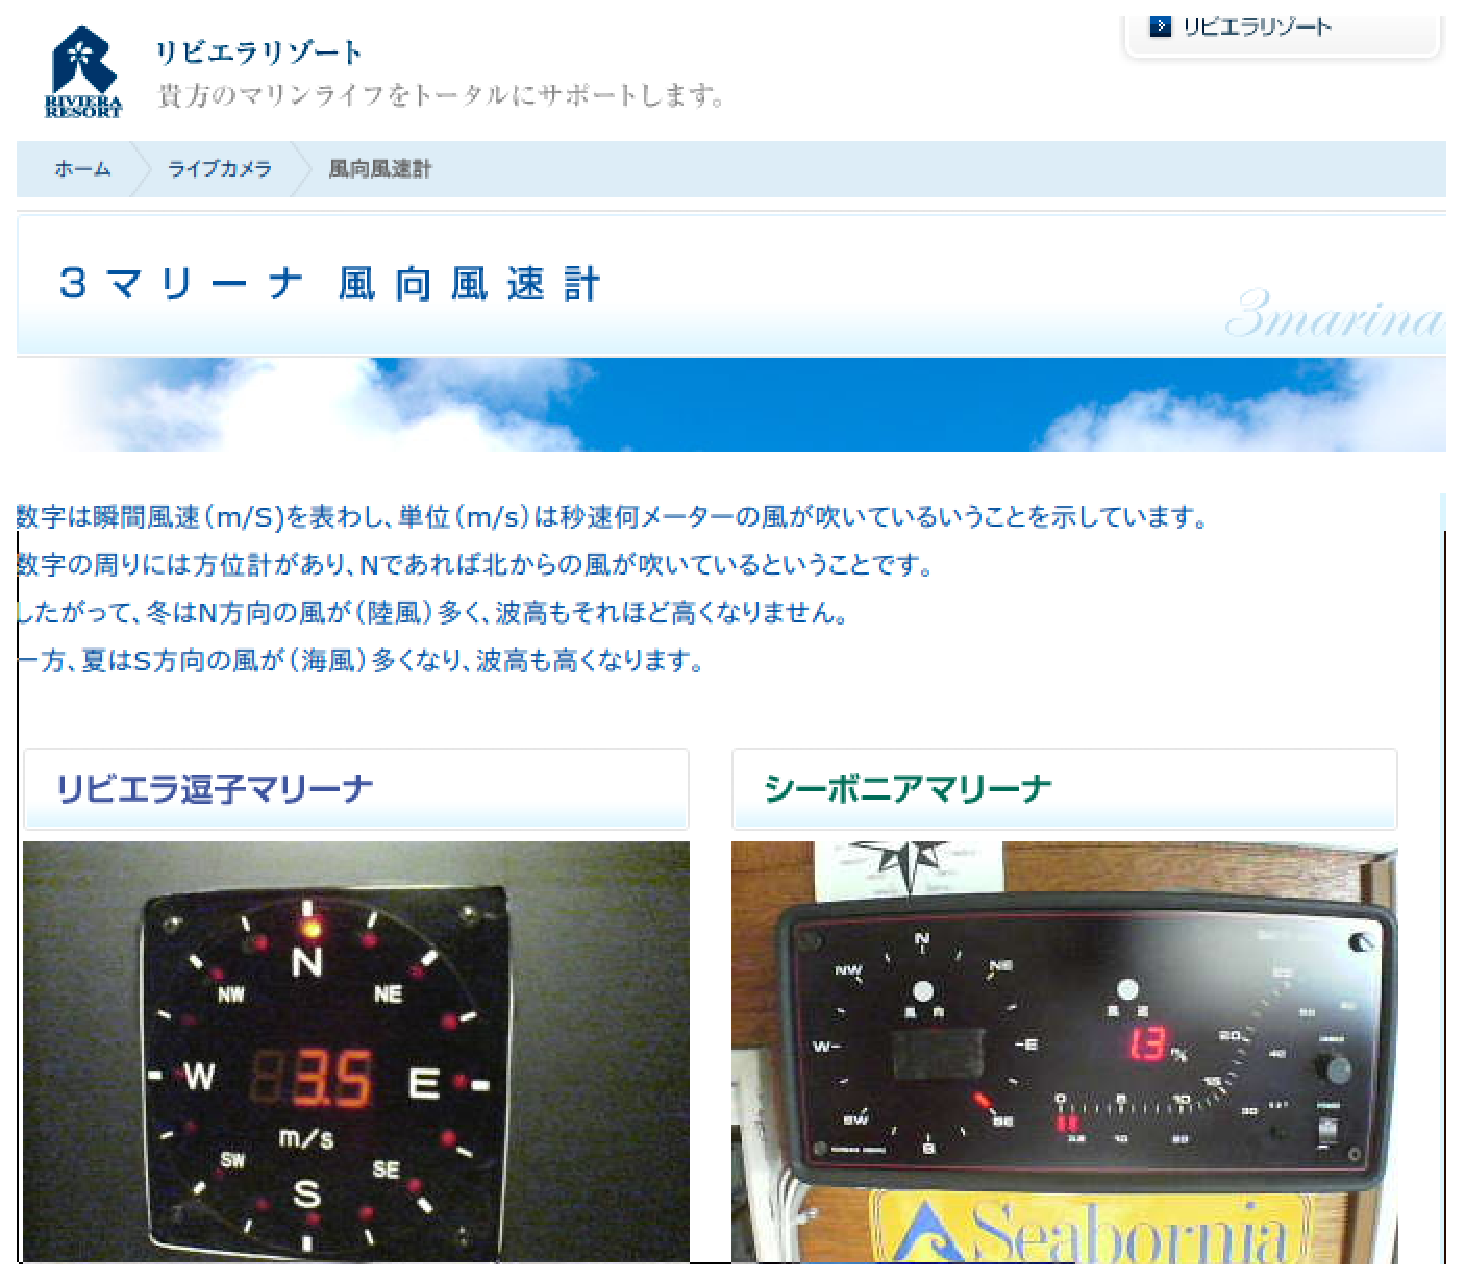
\includegraphics[width=140mm]{image/hayama_wind_large.eps}}
    \end{center}
    \caption{葉山の風速情報}
    \label{fig:hayama_wind}
  \end{minipage}
\end{figure}

\section{今後の展望}

考察で述べた三つの問題に対する解決法を提案する。

一つ目にテキスト形式のデータしか扱う事ができないという問題である。この問題に対してはAndroidクライアントが画像形式のデータを表示する仕様に変更する事で対応出来ると考えられる。サーバーから送られるJSONに画像URLが含まれていれば、それを展開して表示する仕様を実装することで解決できるだろう。

二つ目にプレーンなテキストを並べているだけなので、情報の見やすさや分かりやすさが高いレベルで実現されていないという問題である。
この問題に対しては、センサーから取得した数値データなどであれば閾値を設定し、閾値を超えれば通知領域に通知を出したり表示色を変更することなどで値の変化がわかりやすくなるだろう。
数値ではなくテキストデータであっても、履歴データを保存しておいてそれと照らし合わせ、平常時と違ったデータが検出された場合に通知をしたり、ユーザーが任意にキーワードを設定し、そのキーワードが検出された場合に通知することなどで解決できるだろう。

最後に取得する情報を選択するインターフェースの問題を解決するためにはLindaサーバー上にある情報を予めリスト形式などで表示しておくことが有効であるのではないか。情報のリストからユーザーが選択する方法にすることで、ユーザーはペアを記憶しておく必要がなくなり、更に入力の手間も省くことが出来る。
